% This file was created by matplotlib2tikz v0.6.18.
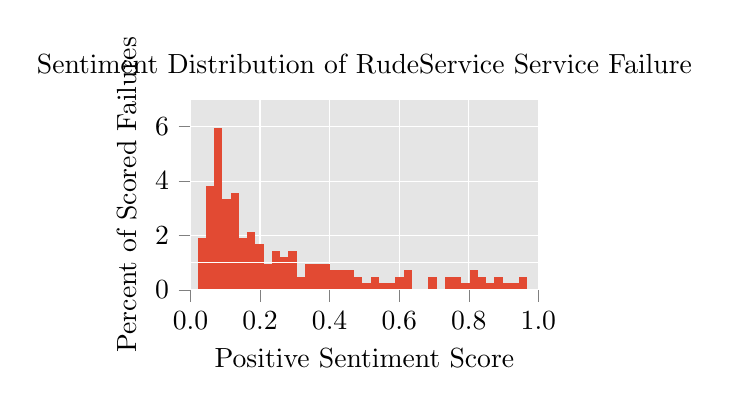
\begin{tikzpicture}

\definecolor{color0}{rgb}{0.886274509803922,0.290196078431373,0.2}

\begin{axis}[
axis background/.style={fill=white!89.80392156862746!black},
axis line style={white},
height=4cm,
tick align=outside,
tick pos=left,
title={Sentiment Distribution of RudeService Service Failure},
width=6cm,
x grid style={white},
xlabel={Positive Sentiment Score},
xmajorgrids,
xmin=0, xmax=1,
xtick={0,0.2,0.4,0.6,0.8,1},
xticklabels={0.0,0.2,0.4,0.6,0.8,1.0},
y grid style={white},
ylabel={Percent of Scored Failures},
ymajorgrids,
ymin=0, ymax=7
]
\draw[fill=color0,draw opacity=0] (axis cs:0.0205376353114843,0) rectangle (axis cs:0.0442337617278099,1.9073892401699);
\draw[fill=color0,draw opacity=0] (axis cs:0.0442337691783905,0) rectangle (axis cs:0.0679298937320709,3.81477848033979);
\draw[fill=color0,draw opacity=0] (axis cs:0.0679298937320709,0) rectangle (axis cs:0.0916260257363319,5.96059043846098);
\draw[fill=color0,draw opacity=0] (axis cs:0.0916260257363319,0) rectangle (axis cs:0.115322150290012,3.33793169505666);
\draw[fill=color0,draw opacity=0] (axis cs:0.115322157740593,0) rectangle (axis cs:0.139018297195435,3.57635426307659);
\draw[fill=color0,draw opacity=0] (axis cs:0.139018282294273,0) rectangle (axis cs:0.162714406847954,1.90738954003237);
\draw[fill=color0,draw opacity=0] (axis cs:0.162714406847954,0) rectangle (axis cs:0.186410531401634,2.14581323253642);
\draw[fill=color0,draw opacity=0] (axis cs:0.186410546302795,0) rectangle (axis cs:0.210106685757637,1.66896479801015);
\draw[fill=color0,draw opacity=0] (axis cs:0.210106670856476,0) rectangle (axis cs:0.233802795410156,0.953694770016187);
\draw[fill=color0,draw opacity=0] (axis cs:0.233802795410156,0) rectangle (axis cs:0.257498919963837,1.43054215502428);
\draw[fill=color0,draw opacity=0] (axis cs:0.257498919963837,0) rectangle (axis cs:0.281195044517517,1.19211846252023);
\draw[fill=color0,draw opacity=0] (axis cs:0.281195044517517,0) rectangle (axis cs:0.304891169071198,1.43054215502428);
\draw[fill=color0,draw opacity=0] (axis cs:0.304891169071198,0) rectangle (axis cs:0.328587293624878,0.476847385008094);
\draw[fill=color0,draw opacity=0] (axis cs:0.328587293624878,0) rectangle (axis cs:0.352283447980881,0.953693570567595);
\draw[fill=color0,draw opacity=0] (axis cs:0.352283447980881,0) rectangle (axis cs:0.375979572534561,0.953694770016187);
\draw[fill=color0,draw opacity=0] (axis cs:0.375979572534561,0) rectangle (axis cs:0.399675697088242,0.953694770016187);
\draw[fill=color0,draw opacity=0] (axis cs:0.399675697088242,0) rectangle (axis cs:0.423371821641922,0.71527107751214);
\draw[fill=color0,draw opacity=0] (axis cs:0.423371821641922,0) rectangle (axis cs:0.447067946195602,0.71527107751214);
\draw[fill=color0,draw opacity=0] (axis cs:0.447067946195602,0) rectangle (axis cs:0.470764070749283,0.71527107751214);
\draw[fill=color0,draw opacity=0] (axis cs:0.470764070749283,0) rectangle (axis cs:0.494460195302963,0.476847385008094);
\draw[fill=color0,draw opacity=0] (axis cs:0.494460165500641,0) rectangle (axis cs:0.518156290054321,0.238423392641899);
\draw[fill=color0,draw opacity=0] (axis cs:0.518156290054321,0) rectangle (axis cs:0.541852414608002,0.476847385008094);
\draw[fill=color0,draw opacity=0] (axis cs:0.541852474212646,0) rectangle (axis cs:0.565548598766327,0.238423692504047);
\draw[fill=color0,draw opacity=0] (axis cs:0.565548539161682,0) rectangle (axis cs:0.589244663715363,0.238423692504047);
\draw[fill=color0,draw opacity=0] (axis cs:0.589244723320007,0) rectangle (axis cs:0.612940847873688,0.476847385008094);
\draw[fill=color0,draw opacity=0] (axis cs:0.612940788269043,0) rectangle (axis cs:0.636636912822723,0.71527107751214);
\draw[fill=color0,draw opacity=0] (axis cs:0.636636972427368,0) rectangle (axis cs:0.660333096981049,0);
\draw[fill=color0,draw opacity=0] (axis cs:0.660333037376404,0) rectangle (axis cs:0.684029161930084,0);
\draw[fill=color0,draw opacity=0] (axis cs:0.684029221534729,0) rectangle (axis cs:0.707725346088409,0.476847385008094);
\draw[fill=color0,draw opacity=0] (axis cs:0.707725286483765,0) rectangle (axis cs:0.731421411037445,0);
\draw[fill=color0,draw opacity=0] (axis cs:0.73142147064209,0) rectangle (axis cs:0.75511759519577,0.476847385008094);
\draw[fill=color0,draw opacity=0] (axis cs:0.755117535591125,0) rectangle (axis cs:0.778813660144806,0.476847385008094);
\draw[fill=color0,draw opacity=0] (axis cs:0.778813719749451,0) rectangle (axis cs:0.802509903907776,0.238423092780505);
\draw[fill=color0,draw opacity=0] (axis cs:0.802509903907776,0) rectangle (axis cs:0.826206028461456,0.71527107751214);
\draw[fill=color0,draw opacity=0] (axis cs:0.826205968856812,0) rectangle (axis cs:0.849902093410492,0.476847385008094);
\draw[fill=color0,draw opacity=0] (axis cs:0.849902153015137,0) rectangle (axis cs:0.873598277568817,0.238423692504047);
\draw[fill=color0,draw opacity=0] (axis cs:0.873598217964172,0) rectangle (axis cs:0.897294342517853,0.476847385008094);
\draw[fill=color0,draw opacity=0] (axis cs:0.897294402122498,0) rectangle (axis cs:0.920990526676178,0.238423692504047);
\draw[fill=color0,draw opacity=0] (axis cs:0.920990467071533,0) rectangle (axis cs:0.944686591625214,0.238423692504047);
\draw[fill=color0,draw opacity=0] (axis cs:0.944686651229858,0) rectangle (axis cs:0.968382775783539,0.476847385008094);
\path [draw=white, fill opacity=0] (axis cs:0,0)
--(axis cs:0,7);

\path [draw=white, fill opacity=0] (axis cs:1,0)
--(axis cs:1,7);

\path [draw=white, fill opacity=0] (axis cs:0,0)
--(axis cs:1,0);

\path [draw=white, fill opacity=0] (axis cs:0,1)
--(axis cs:1,1);

\end{axis}

\end{tikzpicture}